\section{Implementation}
\label{sec:implementation}

We implemented a Transformer-based text classifier from scratch using PyTorch. The model includes core components such as \textbf{Positional Encoding}, \textbf{Multi-Head Attention}, and \textbf{Encoder Layers}, following the original architecture from Vaswani et al.~\cite{vaswani2017attention}. The IMDb dataset was split into 15,000 training, 5,000 validation, and 5,000 test samples, as illustrated in Figure~\ref{fig:split}.

\subsection{Positional Encoding}

Since Transformers lack an inherent notion of token order, we implemented sinusoidal positional encoding. The positional encoding was added to the token embeddings and calculated as follows:
\begin{align}
\text{PE}_{\text{pos}, 2i} &= \sin\left(\frac{\text{pos}}{10000^{2i/d_{\text{model}}}}\right) \\
\text{PE}_{\text{pos}, 2i+1} &= \cos\left(\frac{\text{pos}}{10000^{2i/d_{\text{model}}}}\right)
\end{align}
This was implemented in PyTorch using sine for even indices and cosine for odd indices.

\subsection{Multi-Head Attention}

To enable the model to attend to information from different representation subspaces, we used multi-head attention. For each head, we projected the input into query, key, and value using separate linear layers:
\begin{verbatim}
self.w_q = nn.Linear(d_model, d_model)
self.w_k = nn.Linear(d_model, d_model)
self.w_v = nn.Linear(d_model, d_model)
\end{verbatim}
The scaled dot-product attention was computed as:
\begin{align}
\text{scores} &= \frac{QK^\top}{\sqrt{d_k}} \\
\text{attn\_weights} &= \text{softmax}(\text{scores}) \\
\text{output} &= \text{dropout}(\text{attn\_weights}) \cdot V
\end{align}


\subsection{Transformer Encoder Layer}

The structure follows the standard Transformer encoder design, where the input first passes through a multi-head self-attention layer followed by a residual connection, dropout, and layer normalization. This is then followed by a feed-forward network (FFN), again combined with a residual connection, dropout, and normalization.

\begin{figure}[t]
\centering
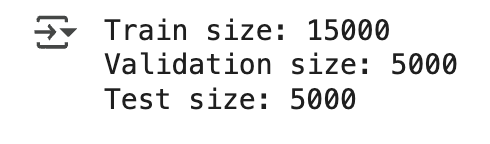
\includegraphics[width=0.7\linewidth]{size.png}
\caption{Dataset split: 15,000 for training, 5,000 for validation, and 5,000 for testing.}
\label{fig:split}
\end{figure}

\section{Discussion}
\label{sec:discussion}

We compare the performance of our self-implemented Transformer with a pre-trained BERT model on the IMDb dataset. The training and evaluation were conducted for a single epoch in both settings. The results reveal a significant performance gap between the two approaches.

As shown in Figure~\ref{fig:transformer_result}, our Transformer model achieved a validation accuracy of 64.20\% and a test accuracy of 64.56\% after one epoch. The corresponding training loss was 0.6638. While this demonstrates that the model learns meaningful representations, the performance is limited due to the lack of pretraining and relatively small model capacity.

\begin{figure}[t]
\centering
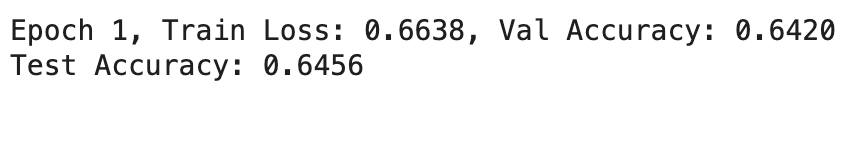
\includegraphics[width=0.85\linewidth]{accuracy.png}
\caption{Training loss and validation/test accuracy of our Transformer model after one epoch.}
\label{fig:transformer_result}
\end{figure}

In contrast, the fine-tuned BERT model achieved a validation accuracy of 81.94\% and a test accuracy of 82.48\%, with a lower training loss of 0.4456 (Figure~\ref{fig:bert_result}). This illustrates the power of transfer learning using pre-trained language models, which leverage large-scale unsupervised learning to capture rich contextual information before task-specific fine-tuning.

\begin{figure}[t]
\centering
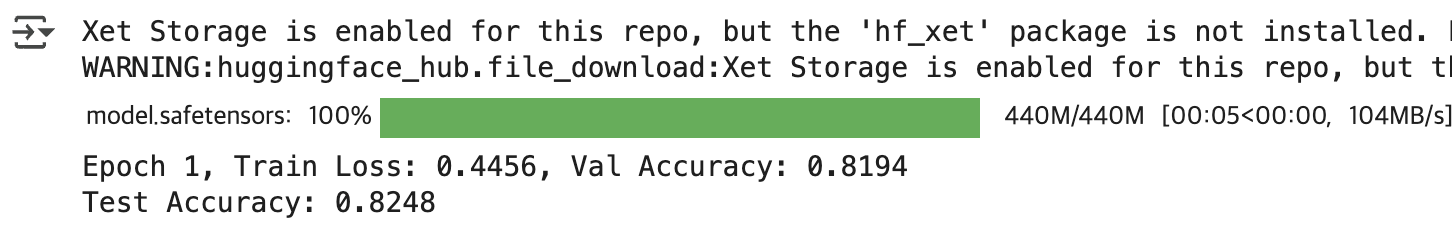
\includegraphics[width=0.85\linewidth]{result.png}
\caption{Training loss and validation/test accuracy of fine-tuned BERT model after one epoch.}
\label{fig:bert_result}
\end{figure}

Overall, this comparison highlights the importance of pretraining in modern NLP tasks. While building a Transformer from scratch is a valuable learning experience, pre-trained models like BERT offer a substantial advantage in terms of accuracy and convergence speed, even with minimal fine-tuning.



